\section{Results}

\subsection{50 Vertices}

When applied to a random graph with 50 vertices, the genetic algorithm finds an optimized solution after around 100 iterations, with a mutation rate of .3, a crossover rate of .99, and 500 chromosomes.

\begin{figure}[H]
\centering
\begin{tabular}{cccccc}
\subfloat[Step 1]{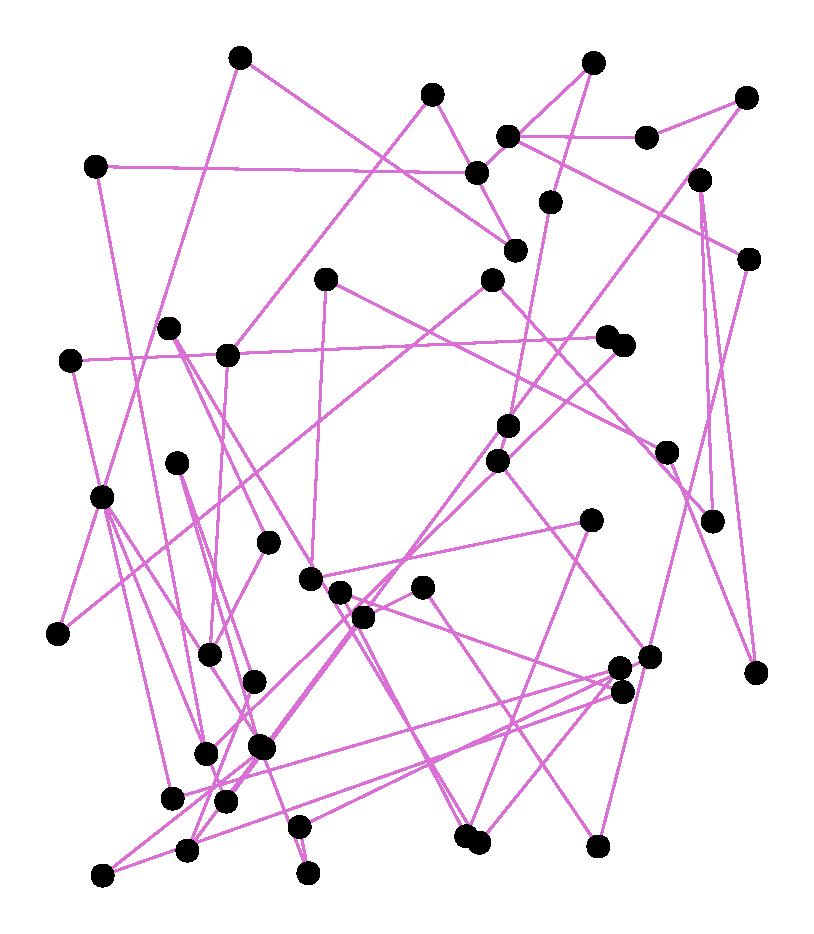
\includegraphics[width = .75in]{images/50/vis_2.pdf}} &
\subfloat[Step 8]{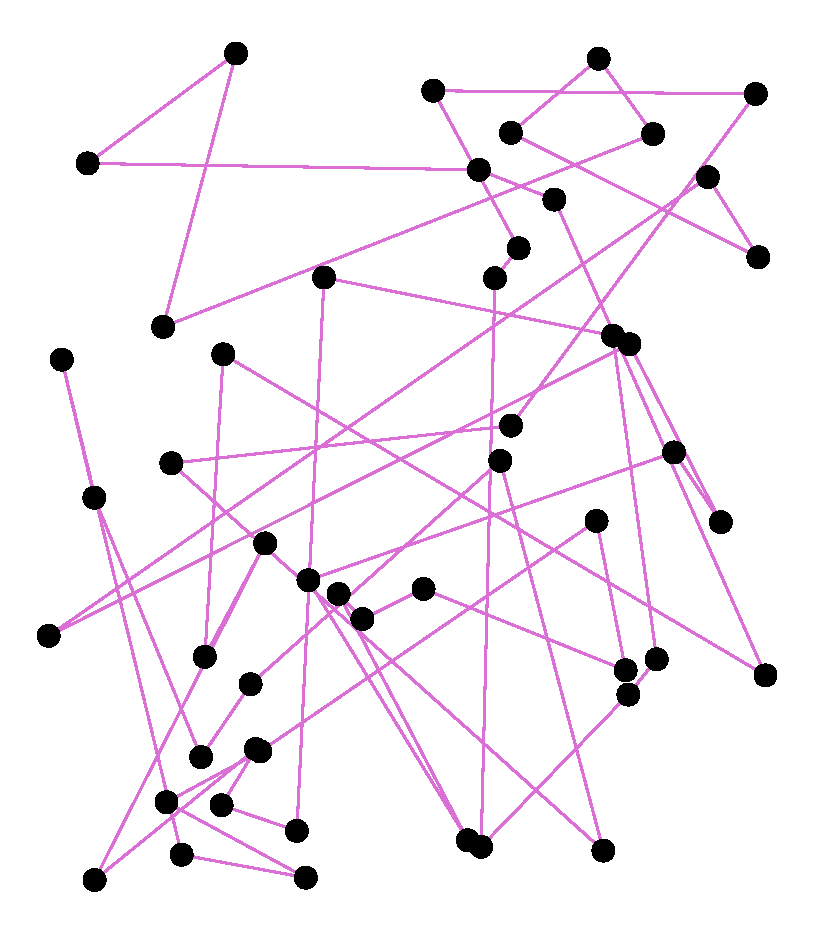
\includegraphics[width = .75in]{images/50/vis_8.pdf}} &
\subfloat[Step 14]{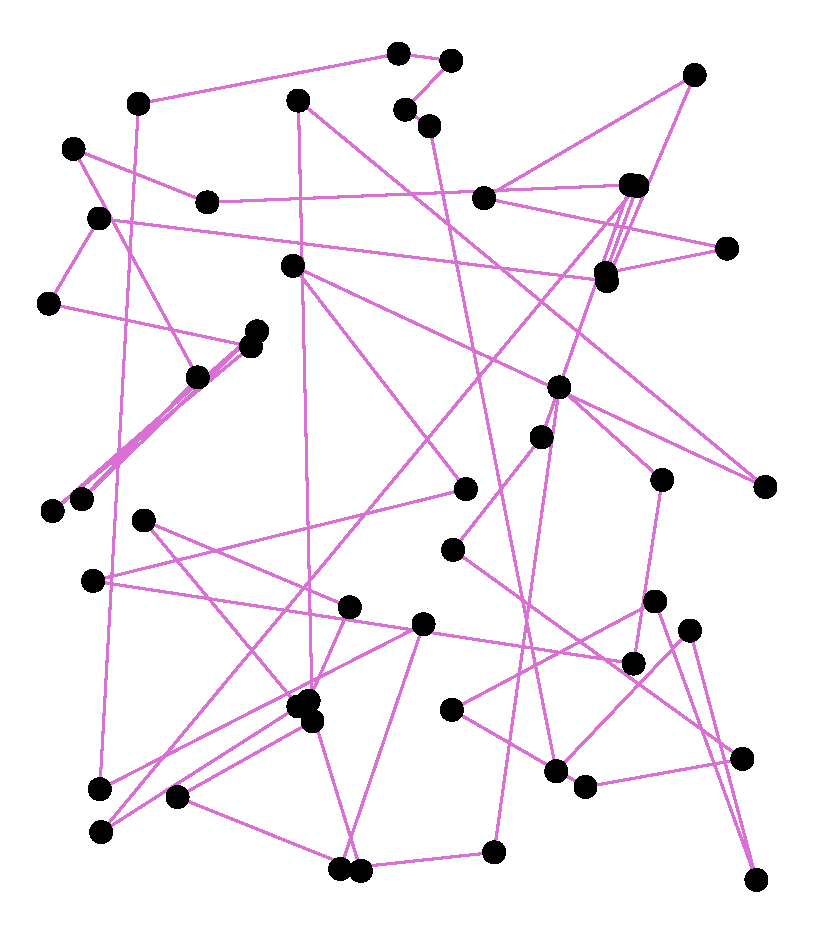
\includegraphics[width = .75in]{images/50/vis_14.pdf}} &
\subfloat[Step 20]{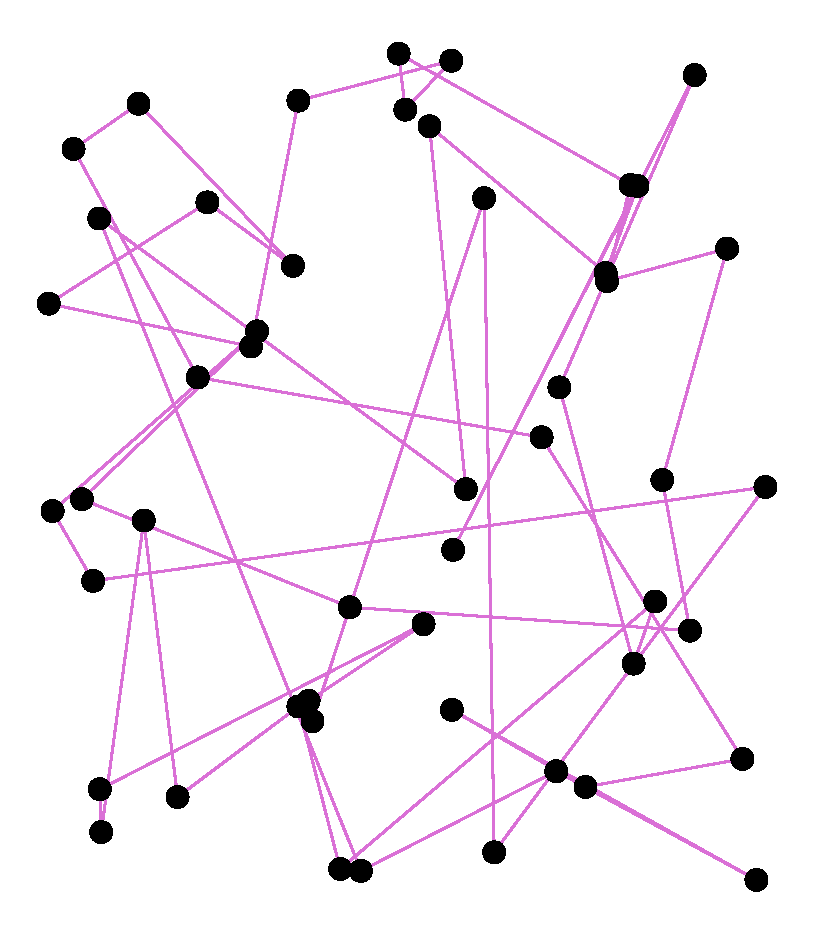
\includegraphics[width = .75in]{images/50/vis_20.pdf}} &
\subfloat[Step 26]{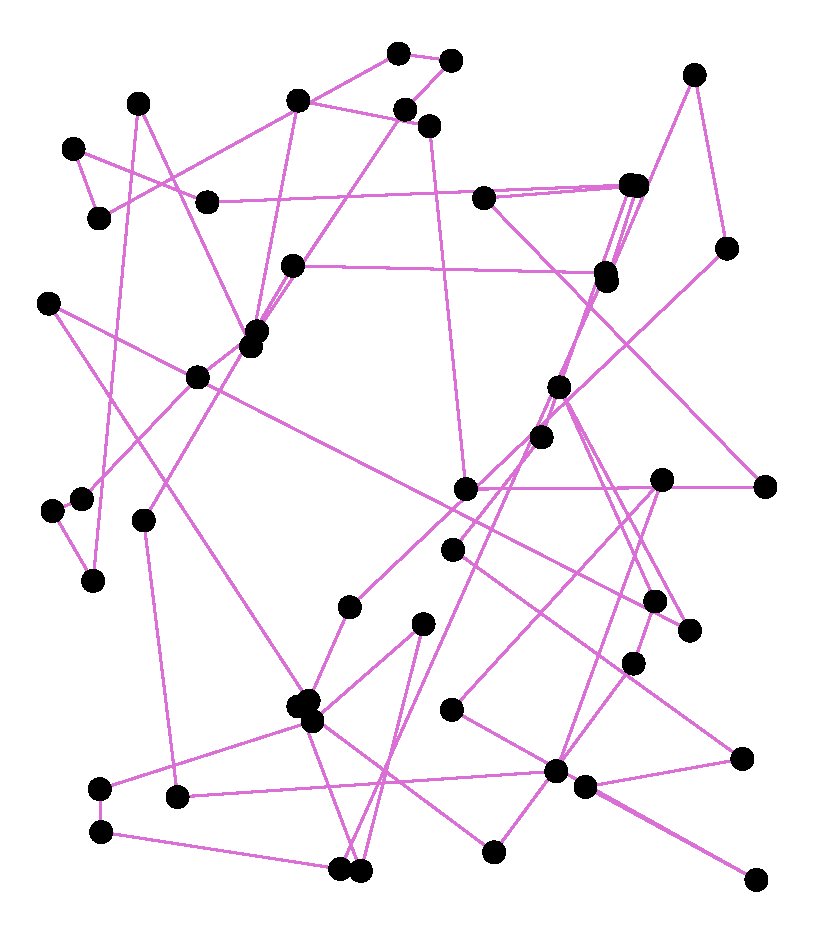
\includegraphics[width = .75in]{images/50/vis_26.pdf}} &
\subfloat[Step 32]{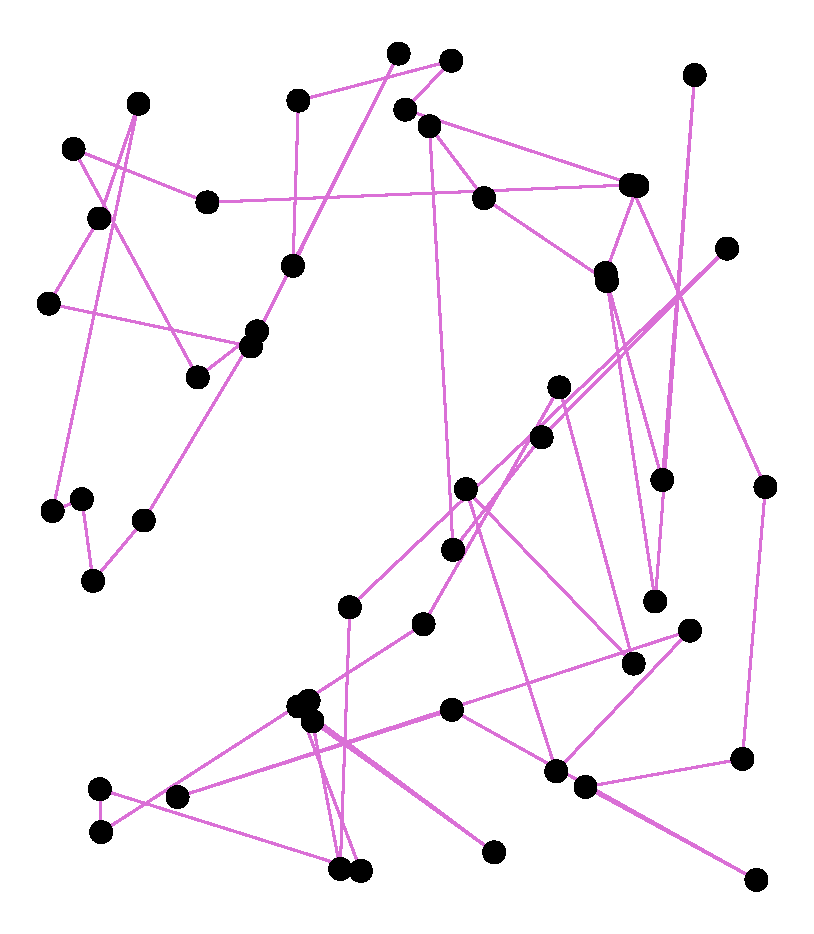
\includegraphics[width = .75in]{images/50/vis_32.pdf}} \\
\subfloat[Step 38]{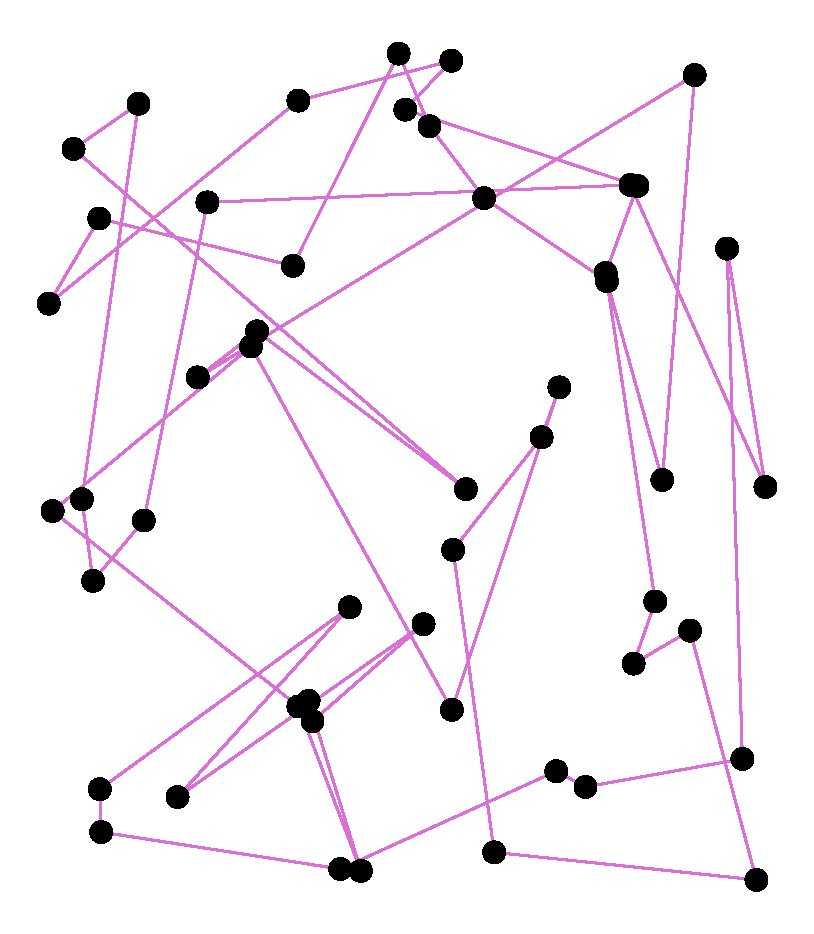
\includegraphics[width = .75in]{images/50/vis_38.pdf}} &
\subfloat[Step 46]{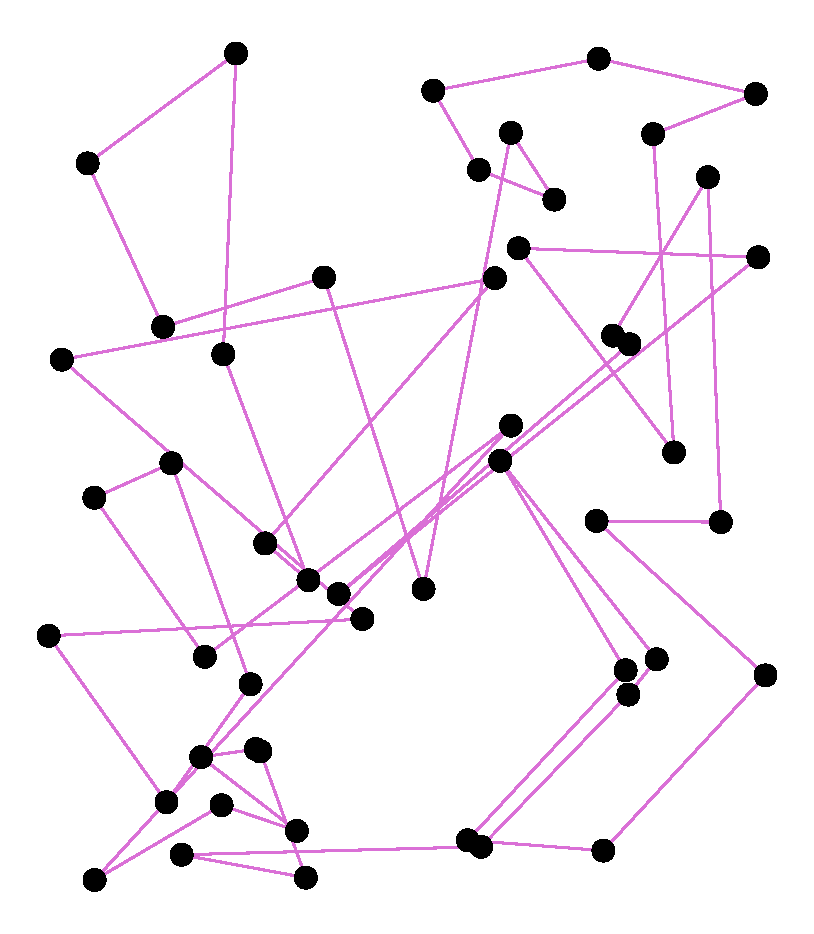
\includegraphics[width = .75in]{images/50/vis_46.pdf}} &
\subfloat[Step 54]{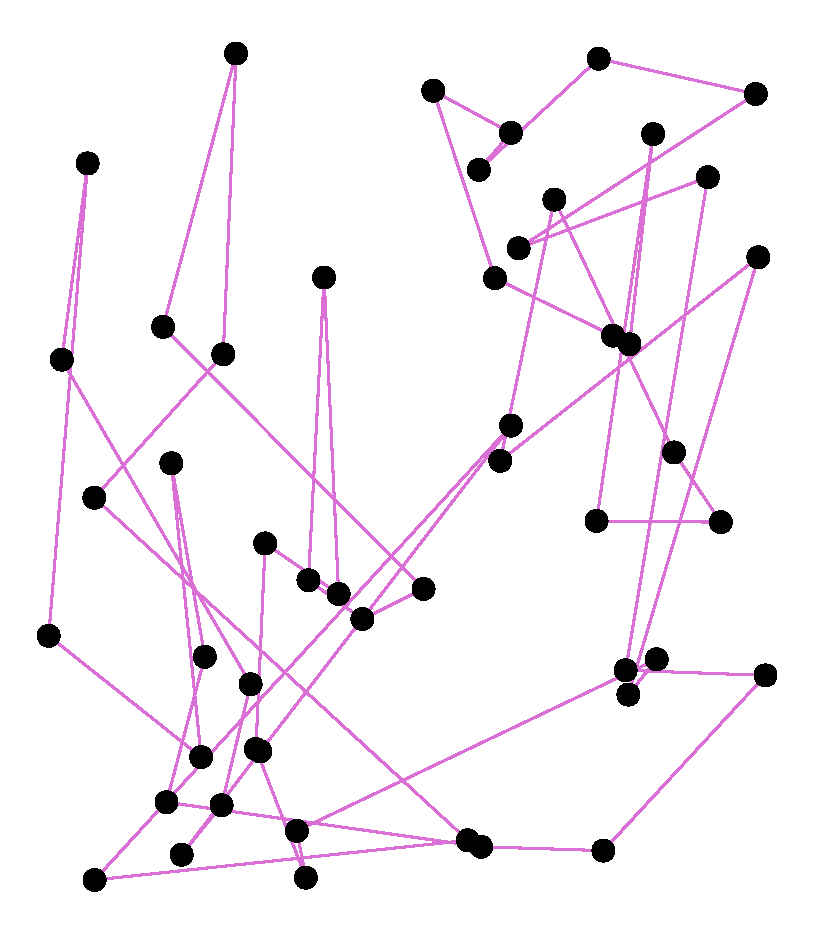
\includegraphics[width = .75in]{images/50/vis_54.pdf}} &
\subfloat[Step 62]{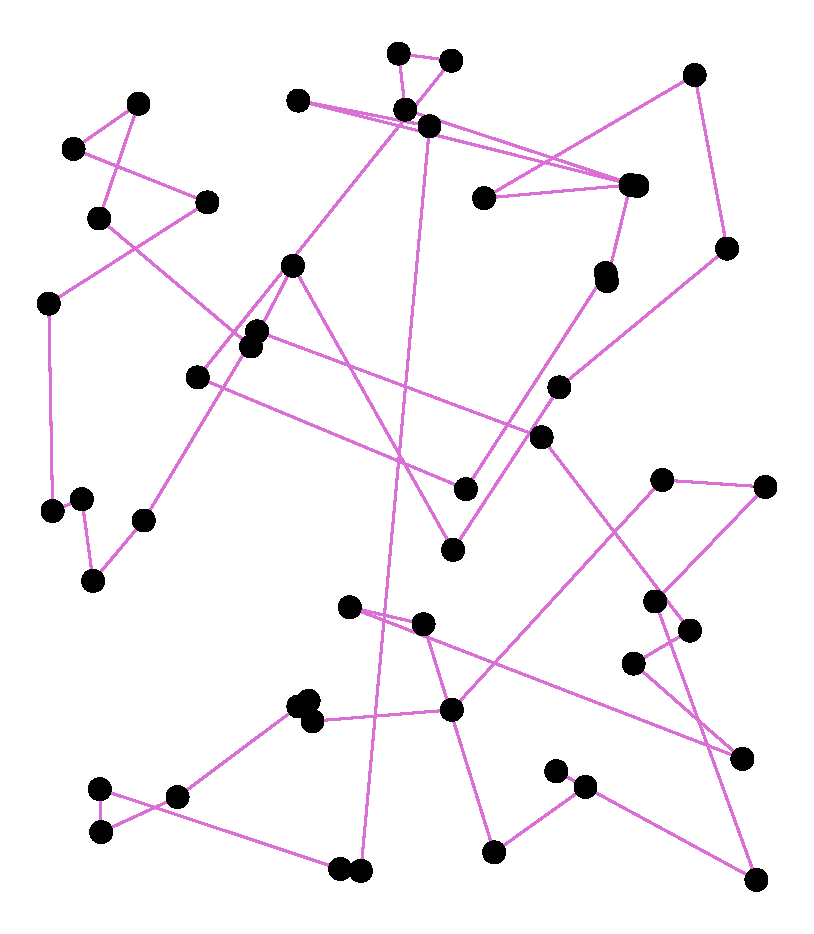
\includegraphics[width = .75in]{images/50/vis_62.pdf}} &
\subfloat[Step 70]{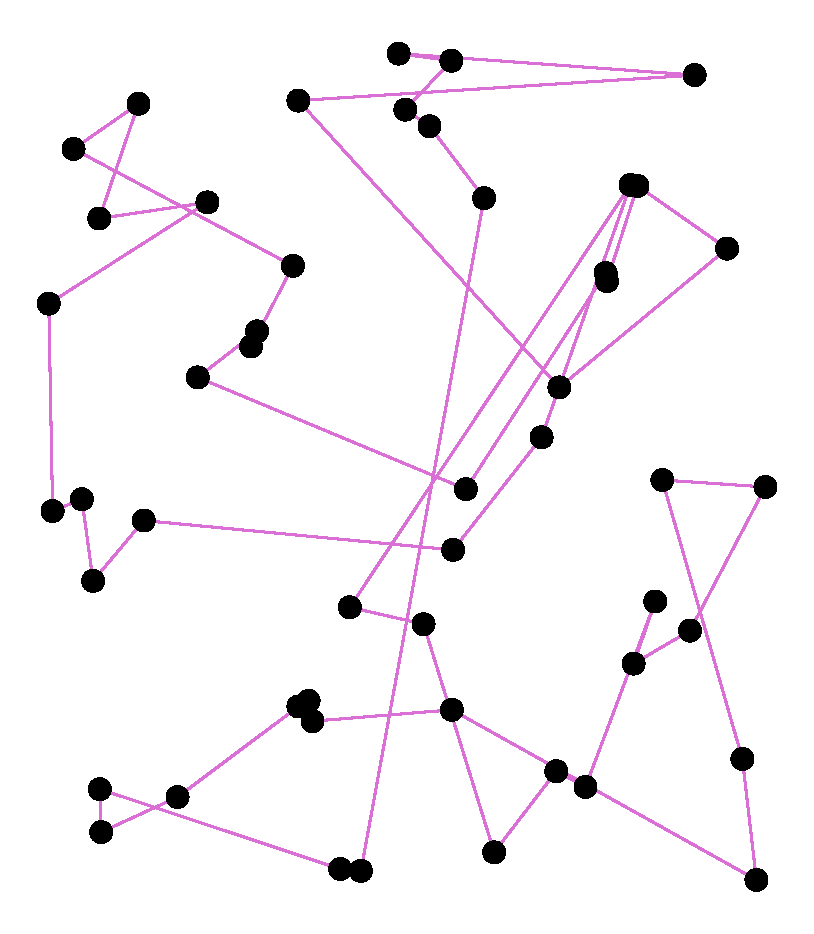
\includegraphics[width = .75in]{images/50/vis_70.pdf}} &
\subfloat[Step 78]{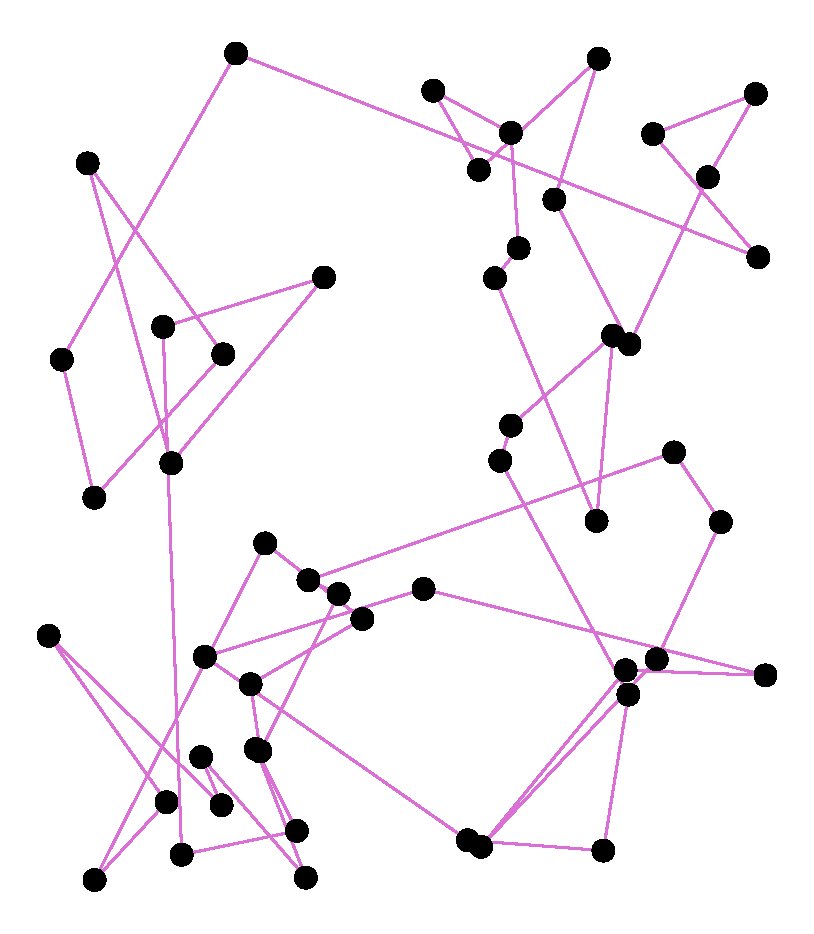
\includegraphics[width = .75in]{images/50/vis_78.pdf}} \\
\subfloat[Step 86]{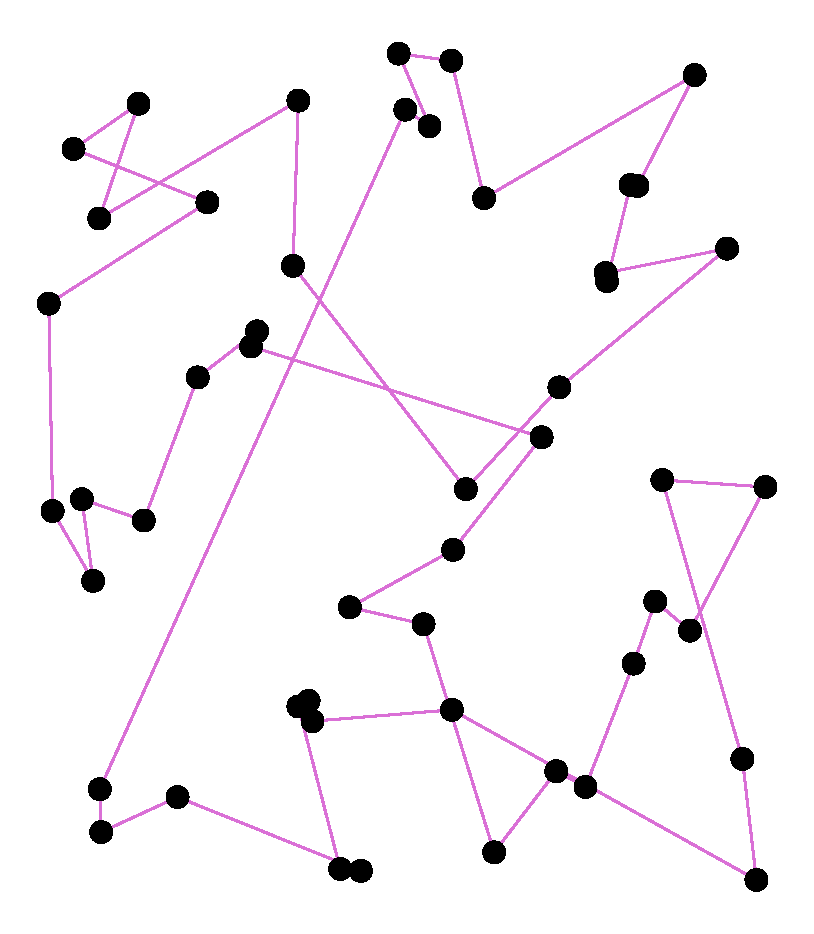
\includegraphics[width = .75in]{images/50/vis_86.pdf}} &
\subfloat[Step 94]{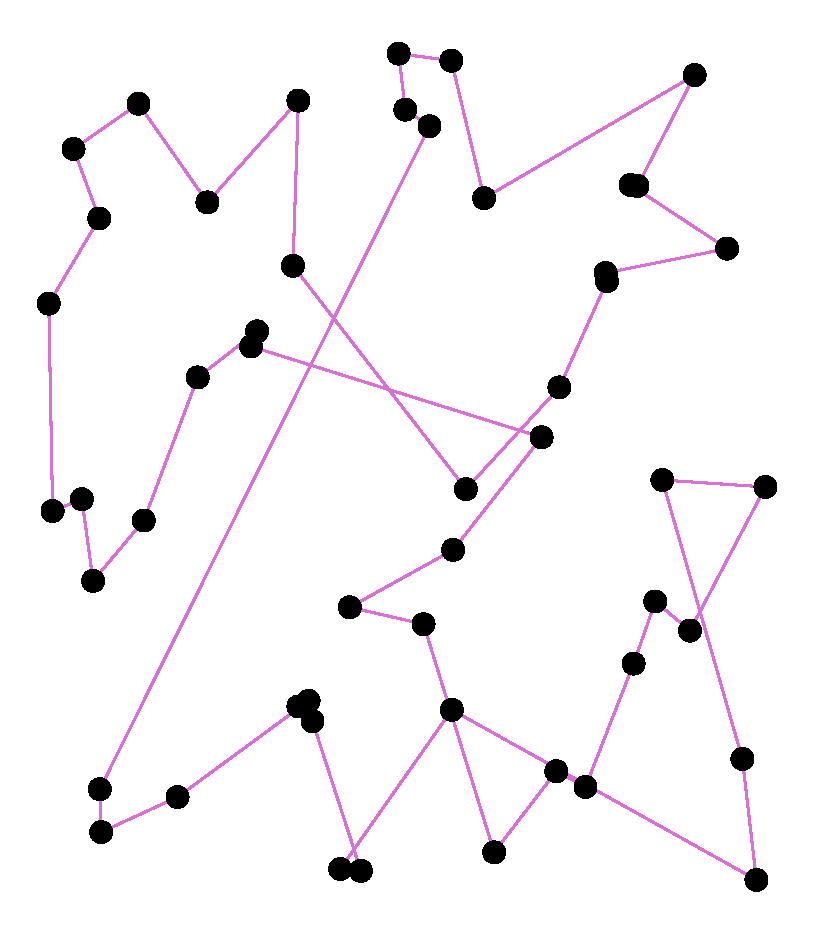
\includegraphics[width = .75in]{images/50/vis_94.pdf}} &
\subfloat[Step 108]{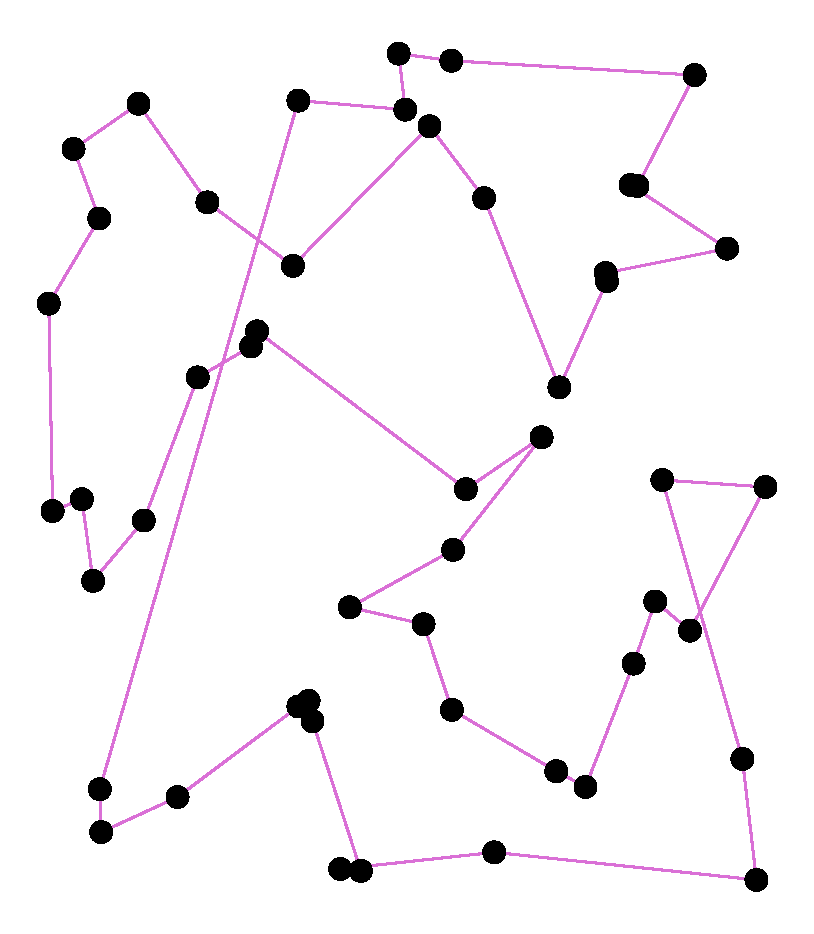
\includegraphics[width = .75in]{images/50/vis_108.pdf}} &
\subfloat[Step 116]{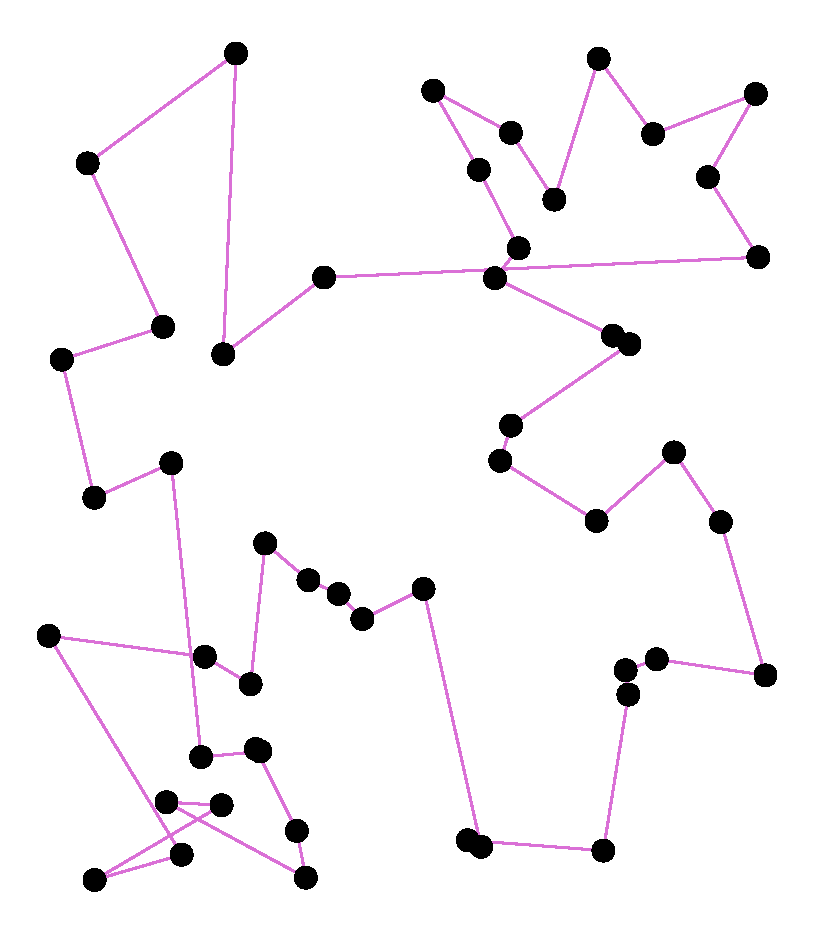
\includegraphics[width = .75in]{images/50/vis_116.pdf}} &
\subfloat[Step 124]{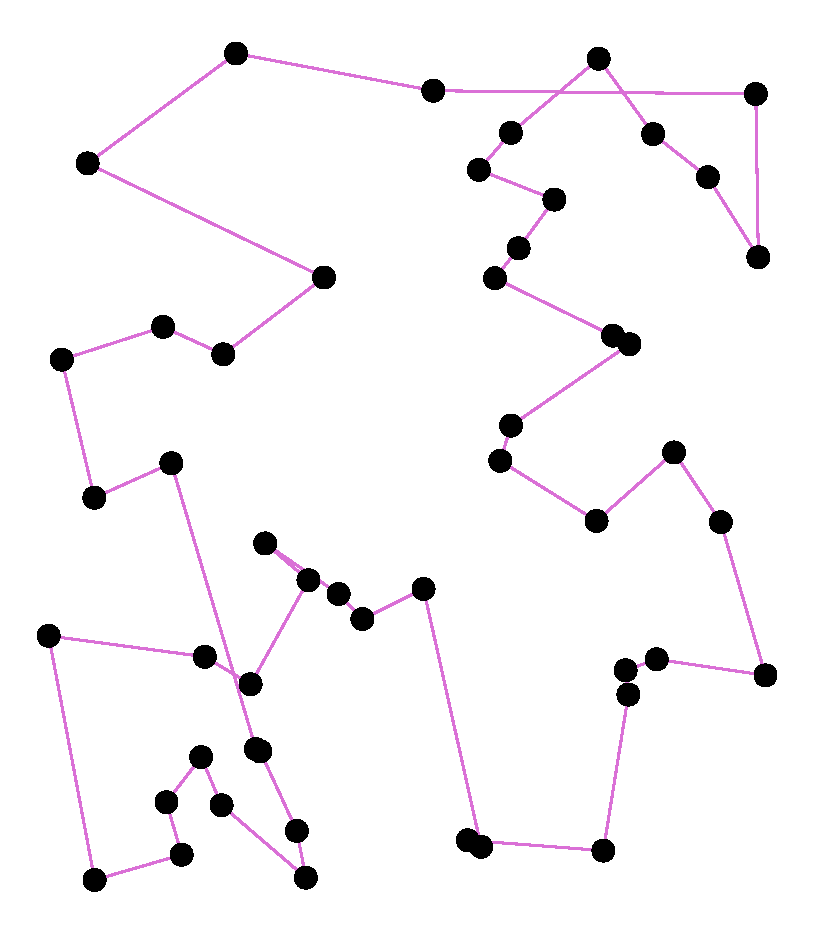
\includegraphics[width = .75in]{images/50/vis_124.pdf}} \\
\end{tabular}
\caption{The genetic algorithm working on an algorithm with 50 vertices.}
\end{figure}

\begin{figure}[H]
\centering
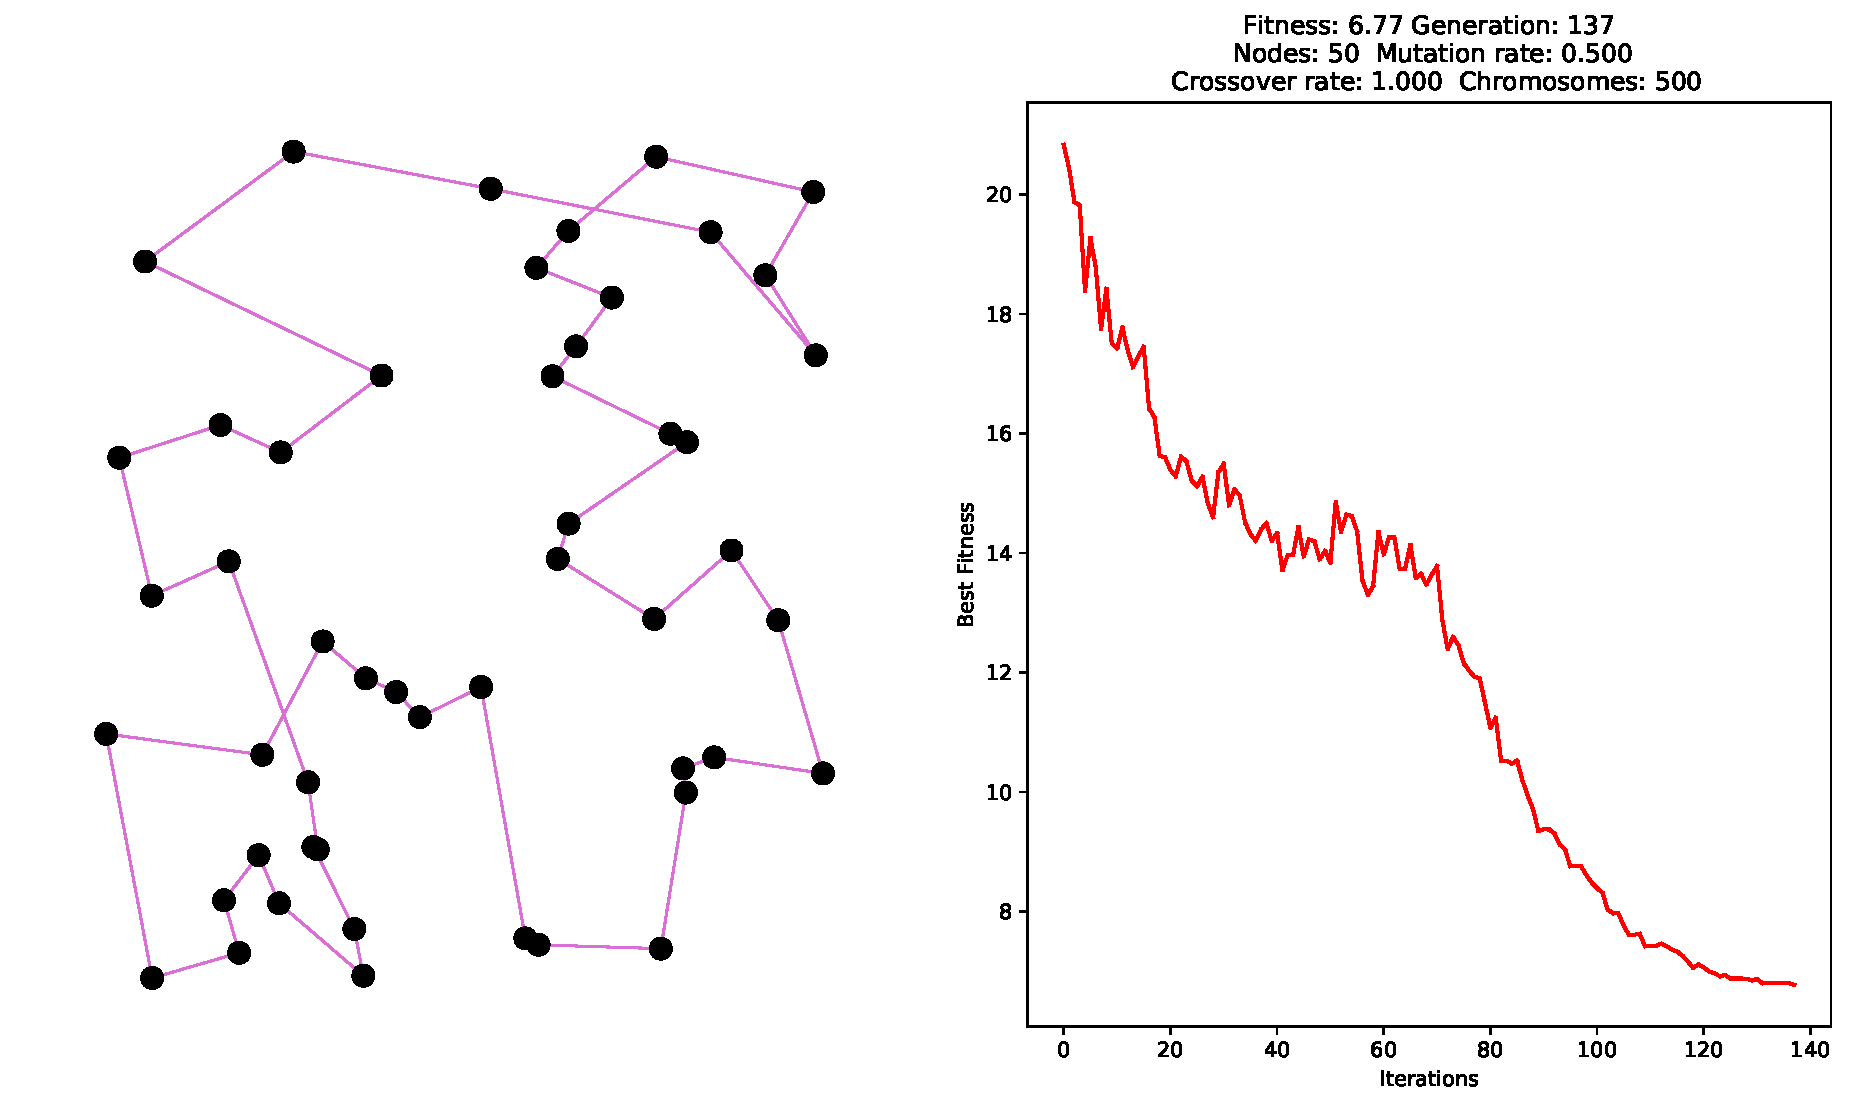
\includegraphics[width=6in]{images/50/graph_138.pdf}
\caption{The genetic algorithm applied to a graph of 50 random vertices, with a mutation rate of .3, a crossover rate of .99, and 500 chromosomes.}
\label{fig:somthing}
\end{figure}

For this example, the genetic algorithm begins with a random solution with fitness of 23 distance units. After 138 iterations, the fittest solution has 7.28 distance units, a 3x improvements.

\subsection{100 Verticess}

At 100 vertices, the algorithm takes longer to optimize, but is able to optimize from 45 distance units in the first iteration to 10.42 in the 650th generation, an improvement of 4.5x.

\begin{figure}[H]
\centering
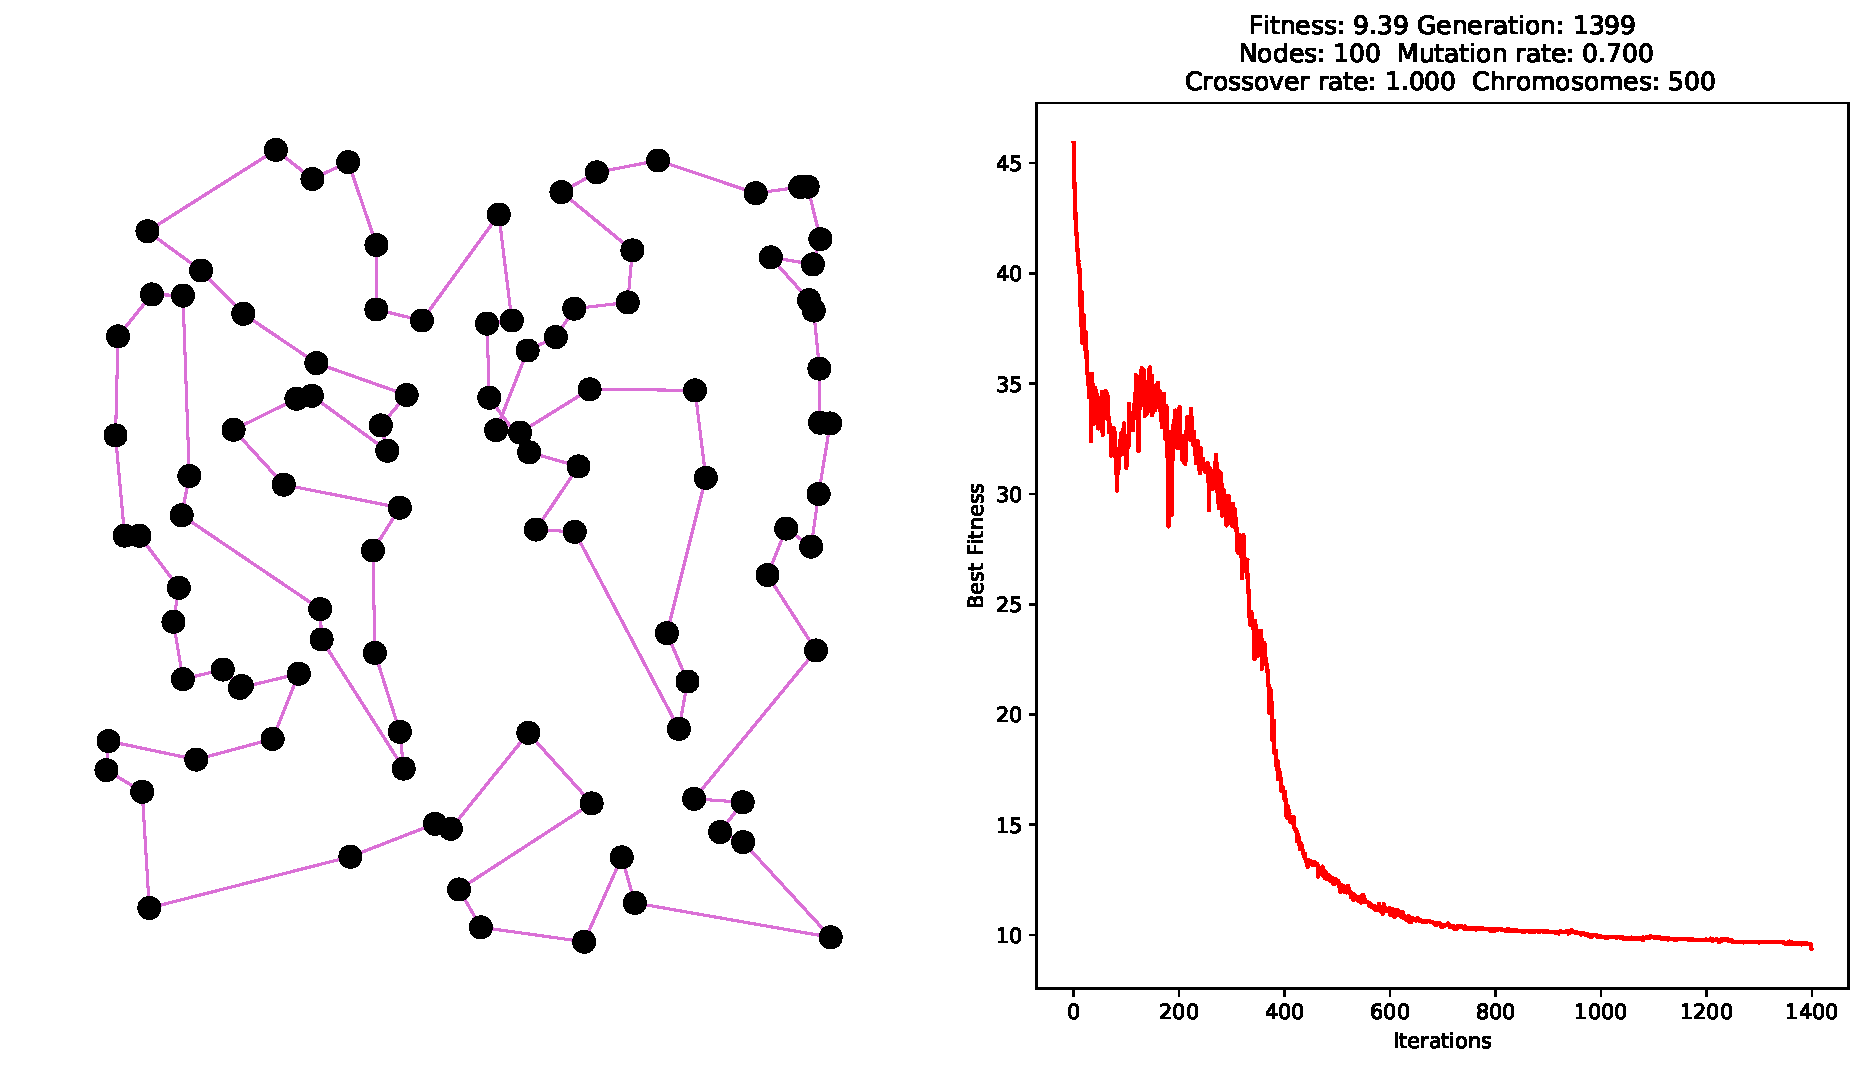
\includegraphics[width=6in]{images/100.pdf}
\caption{The genetic algorithm applied to a graph of 100 random vertices, with a mutation rate of .3, a crossover rate of .99, and 500 chromosomes.}
\label{fig:somthing}
\end{figure}

\subsection{Real-world Dataset}

A great litmus test is a real-world dataset. This dataset is 128 of the largest cities in North America.

\begin{figure}[H]
\centering
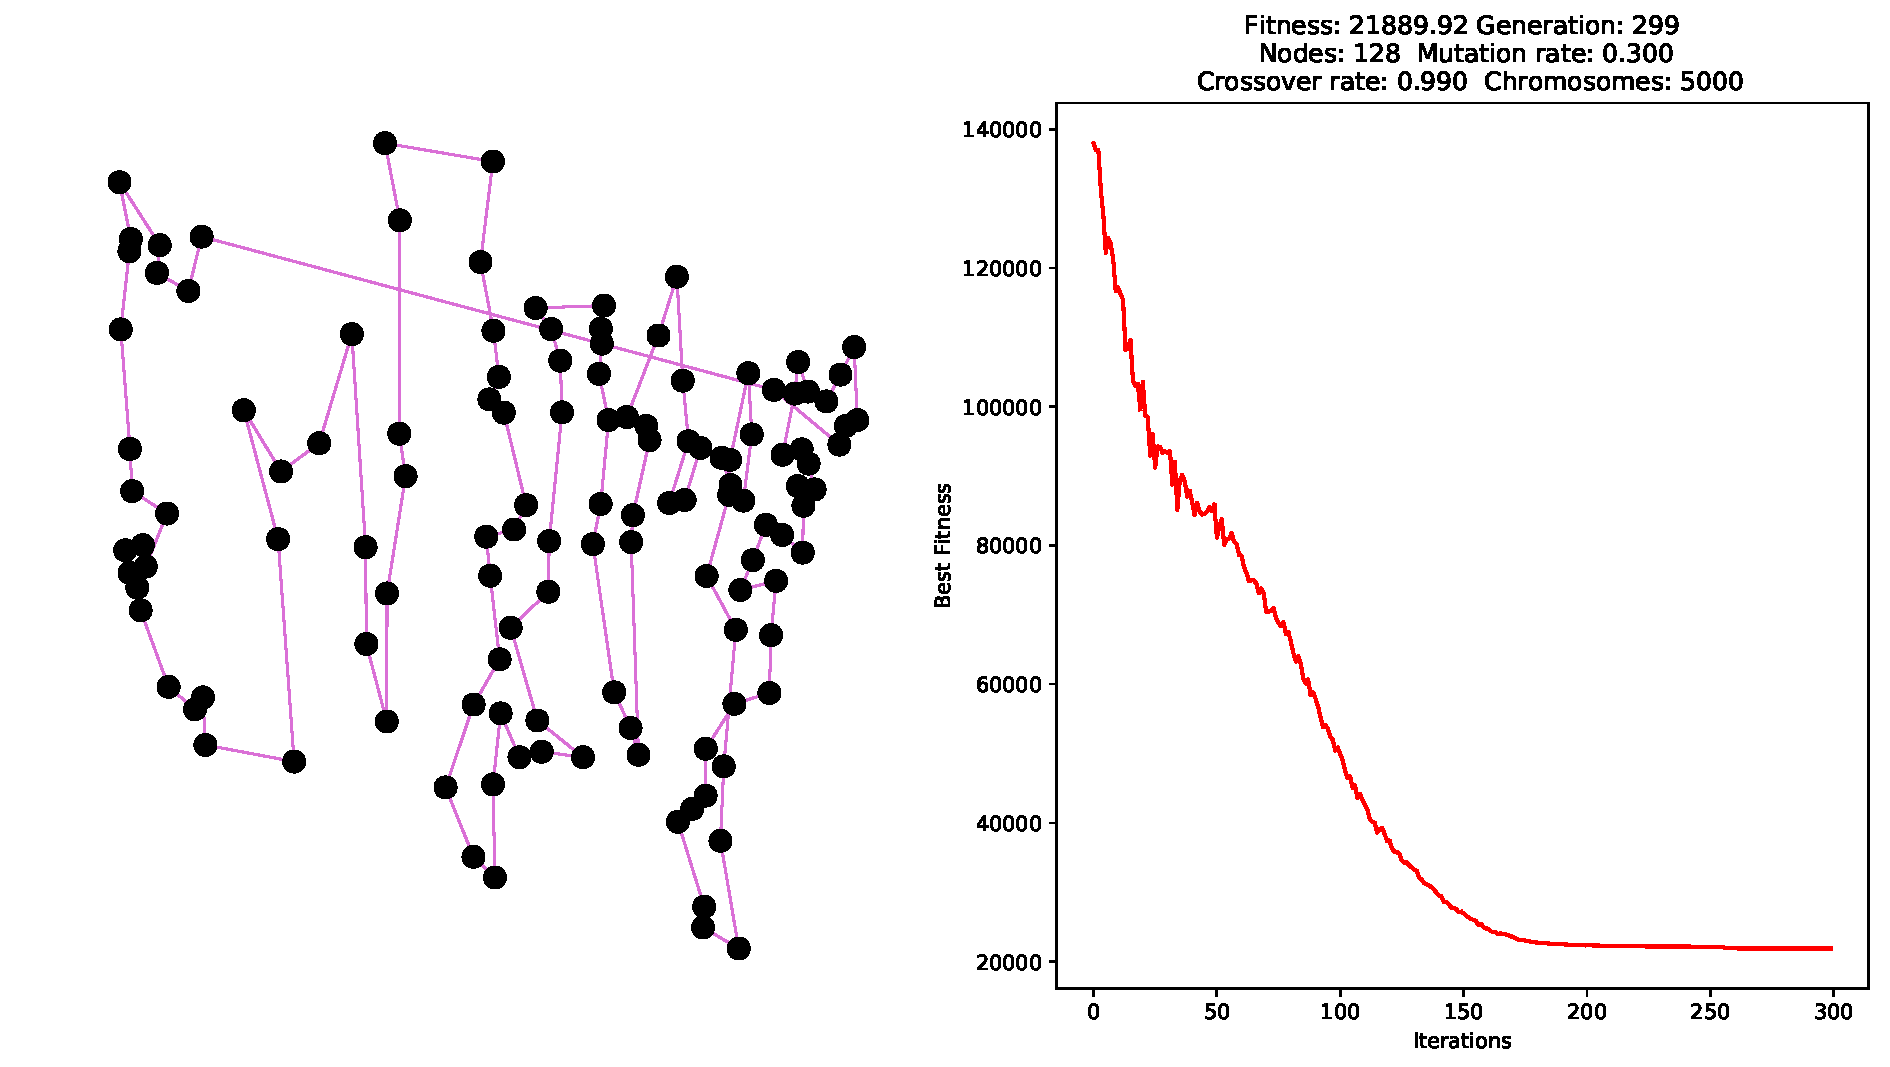
\includegraphics[width=6in]{images/north_america.pdf}
\caption{The genetic algorithm applied to an XY projection of 128 major cities in North America.}
\label{fig:somthing}
\end{figure}